\documentclass[a4paper]{article}

\usepackage{tikz}
\usetikzlibrary{positioning}

\title{PaperTrader Protocol Specification}
\author{altffour}
\date{\today}

\begin{document}
\maketitle
\tableofcontents
\newpage

\section{Introduction}
This is the document for the specification of PaperTrader. PaperTrader is an
application for 'fake' trading assets, to practice investing. The document
contains explainations on how to implement the papertrader application. It 
should be noted that the document isn't `production-ready' until this sentence 
is removed. The document will go over the roles of the master server, and the
worker servers, how they interact with eachother and the communication protocol,
and finally, suggestions on server side implementations.

\section{Overview}
This section contains the required terminology and modelling of the PaperTrader
infrastructure.

\subsection{Terminology}

\subsubsection{Inner World}
This is Master server, and all worker servers. This should be kept under high
lockdown. Meaning, critical data should be kept secure.

\subsubsection{Outer World}
This is the frontend, including the desktop cleint, mobile client, or the
website client. The data here is controlled by the authorization of the account.

\subsubsection{Critical Data}
Cirtical Data are all data types that shouldn't be tampered with without
authorization. For example, accounts, personal information, messages, and in
this context user's portfolios.

\subsubsection{User/Client}
In this context it is the frontend, which is either the desktop client,
mobile client, or the website client.

\subsubsection{User/Client Data}
This is the data of the user. The meaning depends on the specific conext. It
could mean the personal information, credentials, etc. Most of the time it
means data that is attached to a data transfer to identify client (IP?).

\subsubsection{Module}
The module is a set of functions. Usually there would be a main header file
containing the declarations of the functions, a folder with the name of the
header file containing the individual functions definitions of the header file.

\subsubsection{Master Server}
This is the main server that \emph{MUST} be run when deploying the application.
Contains critical data, it would only interact to the outside world by the
worker servers.

\subsubsection{Worker Servers}
These are servers that contact the outer world. Worker Servers will
interact with the Master Server acting like a `cache' servers. Data should be 
routed through worker servers to the master server. The main job for worker 
server is to add timestamps onto commands sent from the user. The data sent to
the main server must contain the data of the client/user. There MUST be ATLEAST
one instance running to have a functional infrastructure.

\subsubsection{User Accounts}
This is the account that abstractly is a the data structure that contains
information about hte user and their account.

\subsection{Infrastructure Model}
A fully deployed infrastructure cotains \emph{ONE} master server, 
\emph{ATLEAST} one worker server, theoretically across the world to maintain 
speed and reliabilty. An overview diagram of the infrastructure: \newline
\begin{center}
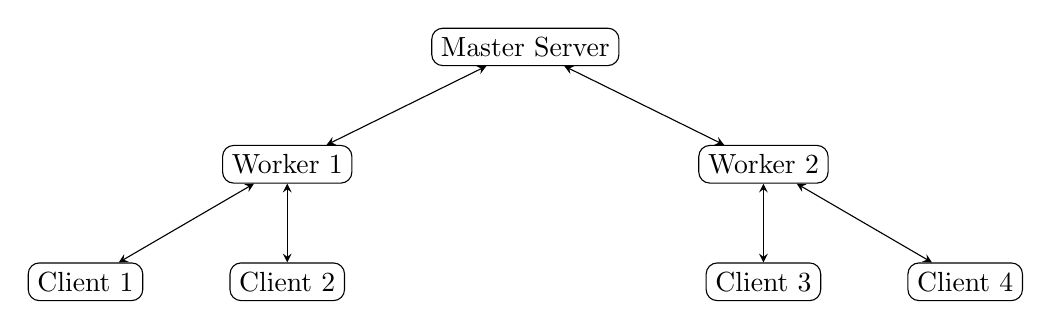
\begin{tikzpicture}[>=stealth,every node/.style={shape=rectangle,draw,rounded 
	corners}]
    % create the nodes
    \node (master) {Master Server};
    \node (worker1) [below left=of master]{Worker 1};
    \node (worker2) [below right=of master]{Worker 2};
	\node (client1) [below left=of worker1]{Client 1};
	\node (client12) [below =of worker1]{Client 2};
	\node (client2) [below =of worker2]{Client 3};
	\node (client22) [below right=of worker2]{Client 4};
    % connect the nodes
    \draw[<->] (master) -- (worker1);
    \draw[<->] (master) -- (worker2);
    \draw[<->] (worker1) -- (client1);
    \draw[<->] (worker2) -- (client2);
    \draw[<->] (worker1) -- (client12);
    \draw[<->] (worker2) -- (client22);
\end{tikzpicture} 
\end{center}

\subsubsection{Master Server Infrastructure Model}
The master can be defined into modules as demonstrated in the following 
diagram: \newline
\begin{center}
	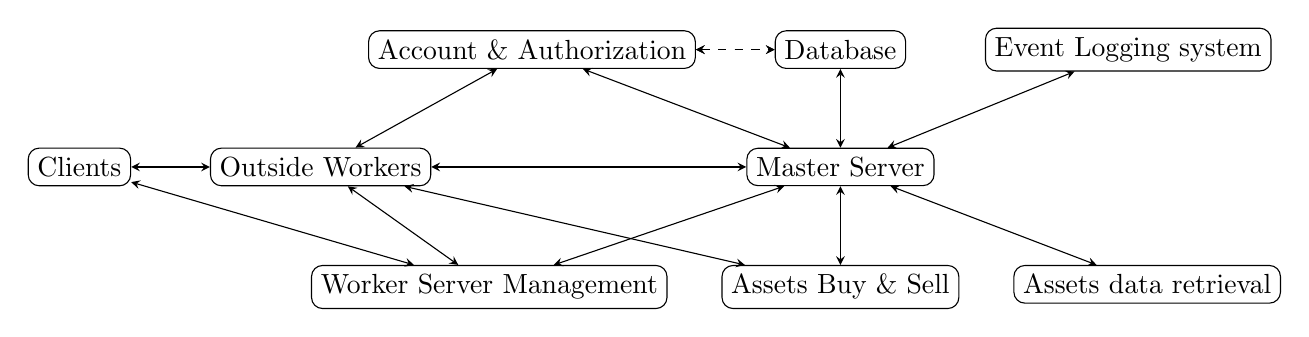
\begin{tikzpicture}[>=stealth,every node/.style={shape=rectangle,draw,
		rounded	corners}]
		% create the nodes.
		\node (master) {Master Server};
		\node (db) [above=of master]{Database};
		\node (acc) [left=of db]{Account \& Authorization};
		\node (log) [right=of db]{Event Logging system};
		\node (worker) [below left=of master]{Worker Server Management};
		\node (asset) [below right=of master]{Assets data retrieval};
		\node (assettrans) [below=of master]{Assets Buy \& Sell};
		\node (outsideworkers) [left=4cm of master] {Outside Workers};
		\node (client) [left=of outsideworkers]{Clients};

		% connect the nodes
		\draw[<->] (outsideworkers) -- (master);
		\draw[<->] (master) -- (db);
		\draw[<->] (master) -- (acc);
		\draw[<->] (acc) -- (outsideworkers);
		\draw[<->, dashed] (acc) -- (db);
		\draw[<->] (master) -- (log);
		\draw[<->] (master) -- (worker);
		\draw[<->] (worker) -- (outsideworkers);
		\draw[<->, dashed] (acc) -- (db);
		\draw[<->] (master) -- (asset);
		\draw[<->] (master) -- (assettrans);
		\draw[<->] (assettrans) -- (outsideworkers);
		\draw[<->] (client) -- (worker);
		\draw[<->] (client) -- (outsideworkers);
	\end{tikzpicture}
\end{center}

\subsubsection{Worker Servers Infrastructure Model}
The worker servers can be defined into modules as demonstrated in the following
diagram:\newline

\begin{center}
	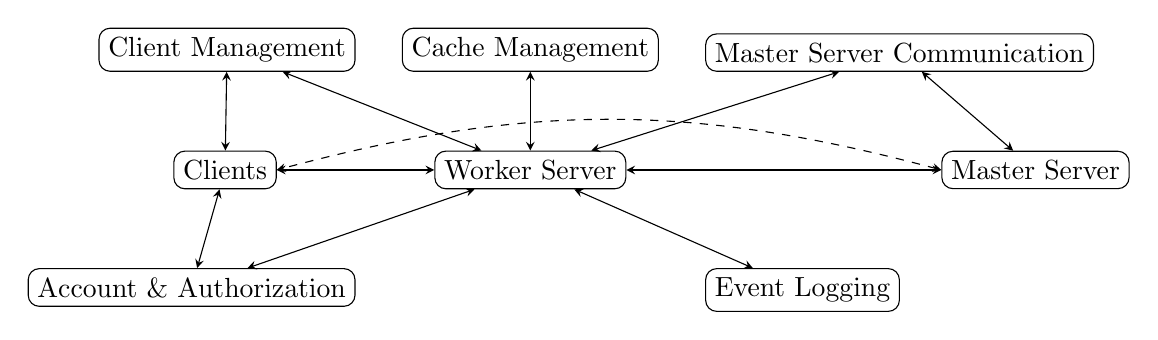
\begin{tikzpicture}[>=stealth,every node/.style={shape=rectangle,draw
		,rounded corners}]
		% create the nodes
		\node (workerserver) {Worker Server};
		\node (masterserver) [right=4cm of workerserver] {Master Server};
		\node (clients) [left=2cm of workerserver] {Clients};
		\node (mastercom) [above right=of workerserver] {Master Server 
			Communication};
		\node (cachemanage) [above=of workerserver] {Cache Management};
		\node (clientmanage) [above left=of workerserver] {Client Management};
		\node (accauth) [below left=of workerserver] {Account \& 
			Authorization};
		\node (event) [below right=of workerserver] {Event Logging};

		% connect the nodes
		\draw[<->] (masterserver) -- (workerserver);
		\draw[<->] (mastercom) -- (masterserver);
		\draw[<->] (workerserver) -- (clients);
		\draw[<->, dashed] (masterserver.west) to [bend right=15] 
		(clients.east);
		\draw[<->] (workerserver) -- (mastercom);
		\draw[<->] (workerserver) -- (cachemanage);
		\draw[<->] (workerserver) -- (clientmanage);
		\draw[<->] (clientmanage) -- (clients);
		\draw[<->] (workerserver) -- (accauth);
		\draw[<->] (accauth) -- (clients);
		\draw[<->] (workerserver) -- (event);

	\end{tikzpicture}
\end{center}

\subsection{Global Deployment Variables}
This section contains an overview of the global deployment variables.

\subsubsection{List of assets to retrieve}
\label{var_list_assets}
This is the list of assets to retrieve using the assets/stocks API. The list
can be available in a file or hard-coded into the implementation.
\subsubsection{Number of Workers}
\label{var_num_worker}
This is the number of workers deployed with the master server. It must be 
atleast one. The worker server preferably should be deployed regionally.
\subsubsection{Memory Size of Log system}
\label{var_log_size}
This is a technical variable, this is the size of the log in memory before it 
being flushed to harddisk. Generally the smaller this is the more disk speed is
required. And the larger it is the more RAM the instance needs and the faster 
it is.
\subsubsection{Stock Data Update Interval}
\label{var_data_update_interval}
This is the interaval of the stock data retrieval. The more this is the faster
the transactions that can occur in a minute. This should be planned perfectly
so that it can maintain the userbase with the API calls.

\subsection{Data/State Structures}
\label{ds_list}
This section will contain an overview of the data structure. The general data
structures discussed here are:
\begin{itemize}
	\item Account Structure
	\item Session Structure
	\item Assets Structure
	\item Transaction Structure
	\item LogEntry Structure
	\item WorkerServer Structure
	\item MasterState Structure
	\item WorkerState Structure
\end{itemize}

\subsubsection{Account Structure}
\label{ds_account}
The account structure is:
\begin{itemize}
	\item UserName - string - 24 MAX CHARS
	\item Email - string - 321 MAX CHARS
	\item isPassword - bool - true
	\item passHash - string
	\item portfolio - Portfolio Structure
	\item transactions - Transaction Structure List
\end{itemize}

\subsubsection{Session Structure}
\label{ds_session}
The session structure is:
\begin{itemize}
	\item sessionID - string
	\item expiryDate - Date
	\item clientIP - IP
	\item isActive - bool
\end{itemize}

\subsubsection{Asset Structure}
\label{ds_asset}
The assets strucure is:
\begin{itemize}
	\item assetSymbol - string
	\item openVal - num
	\item highVal - num
	\item lowVal - num
	\item closeVal - num
	\item volumeVal - num
\end{itemize}

\subsubsection{LogEntry Structure}
\label{ds_logentry}
The LogEntry structure is:
\begin{itemize}
	\item message - string
	\item date - Date
	\item time - Time
	\item filename - string
	\item funcname - string
	\item linenum - num
\end{itemize}

\subsubsection{WorkerServer Structure}
\label{ds_workerserver}
The worker server structure is:
\begin{itemize}
	\item name - string
	\item gpgkey - string
	\item ipaddr - IP
\end{itemize}

\subsubsection{MasterState Structure}
\label{ds_masterstate}
The master state structure is:
\begin{itemize}
	\item workerServers - WorkerServer Structure List
	\item activeSessions - Session Structure List
	\item assetsData - Assets Structure HashMap
	\item logentries - Log Entry Structure List
\end{itemize}

\subsubsection{WorkerState Structure}
\label{ds_workerstate}
The worker state structure is:
\begin{itemize}
	\item masterServersock - Socket
	\item sessions - Session Structure List
	\item logentries - Log Entry Structure List
\end{itemize}

\section{A more Technical Overview}
This is the section that describes the functioning parts of the project in
detail. We will start with modules, including master server modules, and worker
server modules.

\subsection{Master Server}
The master server has multiple modules:
\begin{itemize}
	\item Main Module, i.e the driver.
	\item Database Management.
	\item Account Management.
	\item Event Logging System.
	\item Worker Management.
	\item Assets Data Retrieval.
	\item Assets Transaction Management.
\end{itemize}

\subsubsection{Main Module}
\label{master_mods_main}
The main module should be able to do the following things:
\begin{itemize}
	\item Start the authorization thread.
	\item Start the Worker Management thread.
	\item Start the assets data retrieval thread.
	\item Start the assets transaction thread.
	\item Be able to parse commands from the worker threads.
	\item Be able to route the commands to the correct thread.
\end{itemize}

The main module's functionality in relation of the deployment and running stage
is as follows, The binary containing the master server is run -> initializes 
states required to operate the server -> start the threads -> start listening 
to workers -> parse it -> pass it to the appropriate thread. This is usually 
the set of functions that the main function would call. Putting the workings 
of the main module on a seperate is advised, since it gives the ability to
crash the server and dump the logs from the memory of the event log system.
Refer to \ref{var_log_size} for insight on why this is recommended.

\subsubsection{Database Management}
\label{master_mods_db}
The database management module sould be able to do the following things:
\begin{itemize}
	\item Be able to manipulate files (create, delete, write, read).
	\item Be able to convert data representations (structs) into SQL Databases.
\end{itemize}

The manipulations of files should be quite straightforward, a couple of
functions. The ability to access an SQL database is also necassery.

\subsubsection{Account Management \& Authorization}
\label{master_mods_acc}
The account management \& authorization module  should be able to do the 
following things:
\begin{itemize}
	\item Be able to register new users.
	\item Be able to login \emph{AND} authorize users.
	\item Be able to return a session token for the user.
	\item Be able to manage those session tokens.
\end{itemize}

The module should be able to take the set of information given and put them
into the database (using the database management \ref{master_mods_db}).
All passwords should be hashed and salted, this is up to the implementation on
the exact details. The accounts registered may contain third-party logins ex. 
Google Logins. In that case the account \emph{MUST} be recognized as an account
without a password, and the user should be asked to sign in with the 
third-party credentials. It should also be possible to add a password to the 
account marked to be 'logginable' with third-party logins, making it possible 
to login with the password and using third-party logins.

\subsubsection{Log System}
The log system should be able to do the following things:
\begin{itemize}
	\item To capture the date and time.
	\item To capture the caller's file, function, and line number.
	\item To capture a message and be able to format it.
	\item To be able to store it in a file.
\end{itemize}

One thing should be noted, the log system should not store in memory more 
entries than specified in the global variable: memory size of log system
(\ref{var_log_size}).

\subsubsection{Worker Management}
The worker management module should be able to do the following things:
\begin{itemize}
	\item Keep track of worker servers.
	\item Print information about worker servers.
	\item Retrieve information aobut worker servers.
	\item \emph{ONLY} allow worker servers that are registered.
	\item Verify worker servers with gpg keys.
	\item Able Boot off worker servers while running.
	\item Able to give client list of servers.
\end{itemize}

Most of the functionalities' details can be implementation depended. Keeping
track of worker servers can be done in multiple ways. Printing information can
print stored information about the connected worker server, or retrive 
information about the worker server from the worker server. Should only allow
registered/allowed worker servers to connect to master server AND show in the 
list of available worker servers. Registration should be done using GPG keys.
A list of IPs should be given to the client when a session is connected. The 
list of IPs are the workers' IPs.

\subsubsection{Assets Data Retrieval}
The assets data retrieval model should be able to do the following things:
\begin{itemize}
	\item Retrieve data in intervals of the global variable: data update 
		retrieval interval (\ref{var_data_update_interval}).
	\item Store them in memory and be able to read them (Parsed, into a 
		struct).
	\item Be able to communicate with the assets API.
	\item Retrieve list of assets using API (\ref{var_list_assets})
\end{itemize}

The assets API is upto the implementation. Assets Data should be stored in the
memory and retrieved in a thread-safe manner. This module is preferably to be 
run on a thread.

\subsubsection{Assets Buy \& Sell}
Thie assets buy \& sell module should be able to do the following things:
\begin{itemize}
	\item Buy assets and store them into users' portfolios.
	\item Sell assets and store them into users' portfolios.
	\item Validate transactions of buying and selling.
	\item Log transactions to users profiles.
	\item Process queued transactions per update interval 
		(\ref{var_data_update_interval}).
\end{itemize}

The module should provide functions to apply the above functionality. The
logging is \emph{NOT} to be done with the Log sytem, but rather with storing
them on the account transaction history of the issuer of the transaction. The 
history should be able to show the time of the transaction going through. All 
transaction go through a queue. The queue is cleared every update interval.

\subsection{Worker Server}
The worker server has multiple modules:
\begin{itemize}
	\item Main module. i.e The driver.
	\item Master Server Communication.
	\item Cache Management.
	\item Account Authorization Tunnel.
	\item Event Logging System.
	\item Client Management.
\end{itemize}

\subsubsection{Main Module}
The main module should be able to do the following things:
\begin{itemize}
	\item Start the master server communication thread.
	\item Start the client management thread.
\end{itemize}

The main module's functionality in relation of deployment and running stage is 
as follows, the binary containing the worker server is run -> initializes
states required to operate the worker server -> start the threads -> connect to
master server and authorize with the mater server -> start listening to clients
-> parse it -> pass it to the appropriate thread.

\subsubsection{Master Server Communication}
\label{worker_master_comms}
The master server communication module should be able to do the following:
\begin{itemize}
	\item Parse commands.
	\item Send them to the master server.
\end{itemize}

The parsing is quite important and it is explained further in the document.

\subsubsection{Client Management}
The client management module should be able to do the following:
\begin{itemize}
	\item Keep track of connected clients.
	\item Keep track of sessions.
	\item Be able to give out session tokens to clients.
	\item Be able to verify those session tokens.
	\item Be able to expire those session tokens.
\end{itemize}

Keeping track of the clients data structure is explained in the data structure
section of the document TODO.

\subsubsection{Account Authorization Tunnel}
The account authorization tunnel module should be able to do the following
things:
\begin{itemize}
	\item Recieve the credentials from the client.
	\item Parse the credentails into commands.
	\item Send them to the master server using the master server communication
		module.
	\item Return the login status.
	\item Notify the client management with the new client. Make new token and
		send to client.
\end{itemize}

The account authorization tunnel is simple. Get hte credentials, parse them,
send them to the master server. Wait for reply, if successfully logged in, make
a new session token and send it to the client.

\subsubsection{Logging System}
The log system should be able to do the following things:
\begin{itemize}
	\item To capture the date and time.
	\item To capture the caller's file, function, and line number.
	\item To capture a message and be able to format it.
	\item To be able to store it in a file.
\end{itemize}

One thing should be noted, the log system should not store in memory more 
entries than specified in the global variable: memory size of log system
(\ref{var_log_size}).

\subsubsection{Cache Management}
The cache management module shoudl be able to do the following things:
\begin{itemize}
	\item Keep track of memory pointers, and destroy them correctly.
	\item Efficiently keep track of memory (ex. hash maps).
	\item Store past assets values.
\end{itemize}

This is very closely related to the implementation. It is not a must to have a
cache system, it is recommended though due to the limited number of API calls
to assets/stock values.

\section{The Protocol}
This section will describe the protcol used in PaperTrader.

\subsection{Design Goals}
\begin{itemize}
	\item Based on the TCP protocol.
	\item Connectionless model.
	\item Authorization based communication.
	\item Authentication of commands based on expirable session ID
	\item Optmization to prevent high usage of the stock API (e.x. storing
		asset values, caching data between update intervals).
	\item Parties involved: MasterServer (1), WorkerServers (multiple), clients
		(multiple). 
	\item Parties connections: MasterServer <-> WorkerServers <-> Clients
	\item Basic Error Handling (ex: failed login attempt)
	\item Binary communications, big-endian format.
	\item Message Categories are: Commands, Data Transfer, Control.
	\item Connection States are: commanding, data transfering.
\end{itemize}

Real world examples are given later in the document. This is a brief 
explaination of the design goals. The protocol is based on connectionless model
meaning that each message should be given with a session ID, except for few.
Messages with functionalites like, give stock values, do transactions, etc are
required to have a session ID attached to the message header. Messages with
functionalities like, login new user, register user, do \emph{NOT} require
session IDs. Communication from the worker servers and the master server are
conectionless models. All commands between master server and worker servers
strictly require UUID to be attached to the message. A list of UUIDs are kept 
on the master server. To verify a worker server, the message transmitted should 
be encrypted using GPG keys, the IP is whitelisted, and UUID is verified in the 
previously mentioned UUIDs list. Verification of the clients are simpler since 
it only requires keeping track of the active session IDs. The 
MasterServer-Client communications are very limited, sending the list of
worker servers is the only functionality available to the client from the
master server. States of the communication are handled localy on the reciever 
and transmitter, i.e states switching are indicated by commands and \emph{NOT} 
values in the message itself. Basic error handling is also facilitated, 
examples are forgotten passwords. The communication is an active session ID
between the clients and the worker servers, and is permanent for the worker and
master servers communication connection.

\subsection{States}
\label{states}
There will be two states in any given communication phase:
\begin{itemize}
	\item Command State
	\item Data Transfer State
\end{itemize}

\subsubsection{Command State}
\label{state_command}
The command state will be the begining of all communication phases. In the
command state commands that don't require transfer of Assets/Profile data are
available to command to the worker/master server. These commands include but
not limited to: login, register, purchase asset, sell asset.

\subsubsection{Data Transfer State}
The data transfer state is switchable from the command state. Switching back to
command state is done at the end of the data transfer. The data transfer
commands include but are not limited to: get asset value, get past asset value,
get predicted future asset value.

\subsection{The Connection}
There are multiple types of connections that are running in the program. The
rules for communication are discussed later in this document.
\begin{itemize}
	\item Master-Worker Server Connection
	\item Client-Worker Server Connection
\end{itemize}

\subsubsection{Master-Worker Server Connection}
The connection is a TCP socket listening on port 2048 on the Master server. The
worker server can connect to this port, and after the authentication process
the master-worker server connection is said to be established.

\subsubsection{Client-Worker Server Connection}
The connection is a TCP socket listening on port 2049 on the Worker server. The
clients can connect to this port using any port from their end, and after the
authentication process the client-worker server connection is said to be 
established.

\subsection{Message Structure}
As mentioned before, all messages are in binary, big-endian format. All
messages follow a certain data structure:
\begin{itemize}
	\item messageType - is it a command, data transfer, server return command?
	\item instruction - the integer representation of the instruction/command.
	\item dataSize - the size of the data with the packet.
	\item argumentCount - the amount of arguments passed to the instruction.
	\item data - the data sent with the packet.
\end{itemize}

\subsection{Instructions}
\label{instructions}
The instructions listed in this section are organized into the two states 
explained in \ref{states}, with the addition of the server return instructions.
Instructions and commands are interchangable in this context, not to be 
confused with the command state (\ref{state_command}). The instruction integer 
representation is a detail that is left for the implementation, nevertheless an
important one. The data field of a message structure can be string arguments 
seperated by a space, these kind of datas are sent on the command state with 
command type instructions. Data can also be binary data. \emph{NOTE:} The 
following representation of the instructions are just for the ease of 
understanding and not meant to be used as literal strings passed on the 
network.

\subsubsection{Command State Instructions}
This a list of instructions that can be executed in the command state of a
connection:
\begin{itemize}
	\item login(username, hashedPass, isExpirable)
	\item login(sessionID)
	\item register(username, email, hashedPass)
	\item purchaseAsset(sessionID, name, quantity)
	\item sellAsset(sessionID, name, quantity)
	\item switchState(sessionID, state)
\end{itemize}

\subsubsection{Data Transfer State Instructions}
This is a list of instructions that can be executed in the command state of a
connection:
\begin{itemize}
	\item getAssetInfo(asset)
	\item getAssetValueCurrent(asset)
	\item getAssetValueDay(asset, date)
	\item getAssetValueWeek(asset, date)
	\item getAssetValueMonth(asset, date)
	\item getAssetValueYear(asset, date)
	\item getAssetValueAllTime(asset)
	\item getUserInfo(sessionID, username)
	\item getUserPortfolio(sessionID, username)
	\item getUserTransactionHistory(sessionID, username)
	\item switchState(sessionID, state)
\end{itemize}

\subsubsection{Server Return Instructions}
These instructions are more of return formats. This is a list of instructions 
that can be returned by a server due to a previous instruction:
\begin{itemize}
	\item loginFail
	\item sessionID
	\item registerFail
	\item registerSuccess
	\item purchaseSuccess
	\item purchaseFail
	\item sellSuccess
	\item sellFail
	\item data
\end{itemize}

This is ofcourse not a comprehensive list, and will be updated with further
releases of the application.

\subsection{Overivew of The Instructions}
This would be a comprehensive overview of the instructions mentioned at
\ref{instructions} 

\subsubsection{login(name, hashedPass, isExpirable)}
The `login' instruction is from the set of command state instructions, and does
not require an active session ID to be provided from the worker server. The
first argument is the username of the account, notice that this is not the
email. This username is what will be used to login. The second argument is a
hashed password. This password hashing is up to the implementation to handle.
And the third and last argument is a boolean indicating whether to remember the
sessionID or dispose it after disconnection of the user. The length of the
storing of the session is upto the impelmentation. On success, the server would
return the `sessionID' instruction with the sessionID attached to it. On 
failure, the server would return `loginFail'.

\subsubsection{login(sessionID)}
The `login' instructions is from the set of command state instructions. This
version of the login instruction requires a sessionID. It is used when the
client has already logged and and got a sessionID. The sessionID should be
stored locally on the client's machine. On success, the server would return the
`sessionID' instruction with the same sessionID attached to it. On failure, the
server would return `loginFail'.

\subsubsection{register(username, email, hashedPass)}
The `register' instruction is from the set of command state instructions, and
does not requrie an active session ID to be provided from the worker server.
The first argument is the username of the account, that would be used to login
with. The second argument is the email of the account. The third argument is
the hashed password. The hashing mechanism is up to the implementation. On
success, the server would reurn the `registerSuccess' instruction. On failure,
the server would return the `registerFail' instruction.

\subsubsection{purchaseAsset(sessionID, name, quantity)}
The `purchaseAsset' instruction is from the set of command state instructions,
and requires an active session ID to be provided from and to the worker server.
The sessionID argument will identify the caller of the function. The second
argument is the name of the asset to buy. The third argument is the quantity to
buy. On success, the server would return `purchaseSuccess' instruction. On
failure, the server would return `purchaseFail' instruction with the reason
in the command's arguments.

\subsubsection{sellAsset(sessionID, name, quantity)}
The `sellAsset' instruction is from the set of command state instructionis, and
requires an active sesion ID to be provided from and to the worker server. The
sessoinID argument will identify the caller of the functioni. The second
argument is the name of the asset to sell. The third argument is the quantity
to buy. On success,the server would return `sellSuccess' instruction. On
failure, the server would return `sellFail' instruction with the reason in
the command's arguments.

\end{document}
